\part{Classical statistical mechanics}

\chapter{Classical mechanics}

    In this chapter, we will recall some basic notion of Classical (Hamiltonian) Mechanics.

\section{States, observables, time evolution}
    
    Consider a dynamical system composed by $N$ degrees of freedom in a $d$-dimensional space. A physical state is defined as a point $P$ in a $2dN$-dimensional manifold $\mathcal M^{dN}$, called the phase space, which is the Cartesian product of $N$ single-particle manifolds $\mathcal M^d$. More formally, the phase space is the cotangent bundle $T^*\mathcal C$ of the configuration space $\mathcal C$. In this (smooth) manifold, we locally introduce a chart, which looks like $\mathbb R^{2dN}$, labelled by generalised coordinates $q^i$ and generalised momenta $p_i$, where $i = 1, \ldots dN$. Therefore, a state can be individuated once has been given 
    \begin{equation*}
        \{(q^i, ~p_i)\}_{i=1}^{dN} \in \mathcal M^{dN} ~.
    \end{equation*}
    However, we can combine this $2$ different set of coordinates $q^i$ and $p_i$ into a more convenient single one $\xi_i$ in the following way: 
    \begin{equation}\label{cm:symplcoord}
    \xi^j = \begin{cases}
        q^i & j = 1, \ldots dN \\
        p_i & j = dN+1, \ldots 2dN \\
    \end{cases} ~.
    \end{equation}
    Moreover, we introduce the standard (Lebesgue) measure 
    \begin{equation}\label{cm:measure}
        d\Gamma = \prod_{i=1}^N d^d q^i ~ d^d p_i = \prod_{j=1}^{2N} d^d \xi_j ~.
    \end{equation}
    In the phase space, an observable is a smooth real function 
    \begin{equation*}
        f \colon \mathcal M^{dN} \rightarrow \mathbb R
    \end{equation*}
    and a measurement of this observable at a given time $t_0$ in a fixed point $(q^i(t_0), ~\tilde p_i(t_0))$ is the evaluation of the corresponding function in that point 
    \begin{equation*}
        f = f(q^i(t_0), p_i(t_0)) ~.
    \end{equation*}
    In order to describe time evolution of the system, we need to introduce a special real function $H(q^i, ~p_i, ~t)$, called the Hamiltonian of the system. Through it, we can find how the systems evolve in time by solving the equations of motion, called the Hamilton's equations
    \begin{equation}\label{cm:hameq}
        \dot q^i = \pdv{H}{p_i} ~, \quad \dot p_i = - \pdv{H}{q^i} ~, \quad \text{or} \quad \dot \xi^j = J^{jk} \pdv{H}{\xi^k} ~,
    \end{equation}
    where $J^{jk}$ is the symplectic matrix, a $2N \times 2N$ constant-valued matrix given by
    \begin{equation*}
        J^{jk} = \begin{bmatrix}
            0 & \mathbb I_N \\
            -\mathbb I_N & 0 \\
        \end{bmatrix} ~.
    \end{equation*}

    \begin{example}
        Consider a $1$-dimensional harmonic oscillator of mass $m$ and frequency $\omega$, vibrating around an equilibrium position $q_0$. Its Hamiltonian is given by
        \begin{equation*}
            H (q, p) = \frac{p^2}{2m} + \frac{m \omega^2}{2} (q - q_0)^2 ~,
        \end{equation*}
        while the Hamilton's equations are
        \begin{equation*}
            \dot q = \pdv{H}{p} = \frac{p}{m} ~, \quad \dot p = - \pdv{H}{q} = - m \omega^2 (q - q_0) ~.
        \end{equation*}
    \end{example}
    
    It is important to highlight that the Hamilton's equations are deterministic: once initial conditions $(q^i(t_0), p_i(t_0)) \in \mathcal M^{dN}$ are given, the trajectory in phase space of the system is uniquely and completely determined. This means that there is one and only one trajectory passing through each point of the phase space and two trajectories can never intersect. It is a consequence of the existence and uniqueness theorem of differential equations. 

    \begin{theorem}[Conservation of energy]\label{cm:consen}
        If the Hamiltonian does not depend explicitly on time, it can be interpreted physically as the energy of the system, which is constants
        \begin{equation*}
            H(q^i(t), p_i(t)) = H(q^i(t_0), p_i(t_0)) = E = \text{const} ~.
        \end{equation*}
    \end{theorem}

\section{Probability density distribution}

    Now, we give a few definitions. A macrostate is defined by the knowledge of macroscopic thermodynamic quantities (boundary conditions, like $p, V, N, T, \ldots$); whereas a microstate is defined by the knowledge of the microscopic behaviour of the system in the phase space $(q^i, p_i)$, which is fixed by the initial conditions. However, in general, there are more microstates associated to the same macrostates, since the information carried by a microstate is much more than the one carried by a macrostate. Intuitively, we can say that a system in a defined macrostate can be represented not by only one but by several microstates. This gives rise to the concept of ensemble. We fixed a macrostate set-up, we created a large amount of copies of the same physical system and we look at the different microstate that can represent this macrostate. Mathematically, it can be studied with the introduction of a probability density distribution 
    \begin{equation*}
        \rho(q_i(t), p_i(t),t) \colon \mathcal M^{dN} \rightarrow \mathbb R^+ ~,
    \end{equation*}
    such that it satisfies the following properties
    \begin{enumerate}
        \item positivity, i.e.
        \begin{equation*}
            \rho(q_i, ~p_i, ~t) \geq 0 ~,
        \end{equation*}
        \item normalisation, i.e.
        \begin{equation}\label{cm:norm}
            \int_{\mathcal M^n} \prod_{i=1}^N d^d q_i d^d p_i ~ \rho(q_i, p_i, t) = \int_{\mathcal M^n} d\Gamma ~ \rho(q_i, p_i, t) = 1 ~.
        \end{equation}
    \end{enumerate}
    The probability to find the system in a finite portion of the phase space $\mathcal U \subset \mathcal M^{dN}$ is 
    \begin{equation*}
        \int_{\mathcal U} d\Gamma ~ \rho(q_i, ~p_i, ~t) ~.
    \end{equation*}

    Notice that there is a dimensional problem: a measure must be dimensionless but the measure we have introduced into the phase space $d\Gamma$ has the dimension of an action at the power of $dN$, i.e. $[d\Gamma] = [E]^{dN} [t]^{dN}$. To solve this problem, we introduce an ad hoc constant $h$, called the scale factor, which leads is to a dimensionless volume element
    \begin{equation*}
        d \Omega = \frac{d\Gamma}{h^{dN}} = \frac{\prod_{i=1}^N d^d q^i d^d p^i}{h^{dN}} ~.
    \end{equation*}

\section{Liouville's theorem}

    Given $2$ functions of the phase space $f(q^i, p_i)$ and $g(q^i, p_i)$, we can define a bilinear mapping, called the Poisson's brackets, defined by as
    \begin{equation}\label{cm:poi}
        \{f, g\} = \pdv{f}{q^i} \pdv{g}{p_i} - \pdv{f}{p_i} \pdv{g}{q^i} = \pdv{f}{\xi^j} J^{jk} \pdv{g}{\xi^k} ~,
    \end{equation}
    such that it satisfies the following properties, $\forall h(q^i, p_i)$
    \begin{enumerate}
        \item antisymmetry, i.e.
        \begin{equation*}
            \{f,g\} = - \{g, f\} ~,
        \end{equation*}
        \item Leibniz rule, i.e.
        \begin{equation*}
            \{f, gh\} = g \{f, h\} + \{f, g\} h ~,
        \end{equation*}
        \item Jacobi identity, i.e.
        \begin{equation*}
            \{f , \{g, h\}\} + \{g , \{h, f\}\} + \{h , \{f, g\}\} = 0  ~.
        \end{equation*} 
    \end{enumerate}
    Notice that the symplectic matrix can be defined by the Poisson brackets
    \begin{equation*}
        \{\xi^j, \xi^k \} = J^{jk} ~.
    \end{equation*}
    A canonical transformation $\xi \rightarrow \eta$ is a transformation of the phase space coordinates that preserve the structure of the Poisson's brackets 
    \begin{equation*}
        \{\xi^j, \xi^k\} = \{\eta^j, \eta^k\} = J^{jk} ~.
    \end{equation*}

    To a system of first-order differential equations, like the Hamilton's ones, we can associate an Hamiltonian flow generated by the Hamiltonian vector field
    \begin{equation*}
        \mathbf H = J^{jk} \pdv{H}{\xi^k} \pdv{}{\xi^j} ~.
    \end{equation*}
    Physically, with a fluid analogy, it keeps track of the motion of all particles.
    \begin{theorem}
        Time evolution governed by the Hamilton's equations is a canonical transformation.
    \end{theorem}
    \begin{theorem}
        Canonical transformations preserve volumes in phase space.
    \end{theorem}
    \begin{proof}
        A canonical transformation can be written as 
        \begin{equation*}
            J^{ab} = \{\eta^a, \eta^b\} = \pdv{\eta^a}{\xi^j} J^{jk} \pdv{\eta^b}{\xi^k} ~.
        \end{equation*}
        Now, we compute the determinant of this expression, observing that $M = \partial \eta / \partial \xi$ is the Jacobian matrix of this transformation, and we obtain, using the properties of the determinant
        \begin{equation*}
            \det J = \det (M J M^T) = \det^2 M \det J ~,
        \end{equation*}
        hence 
        \begin{equation*}
            |\det J| = 1 ~.
        \end{equation*}
    \end{proof}

    Combining the last $2$ theorems, we can state an important theorem, named after Liouville. 
    \begin{theorem}[Liouville]
        The volume through the (Hamiltonian) flow generated by the Hamilton's equations is constant
        \begin{equation*}
            \vol \Omega(t_0) = \vol \Omega(t) ~.
        \end{equation*}
        See Figure~\ref{fig:liou}.
    \end{theorem}
    \begin{figure}[h!]
        \centering
        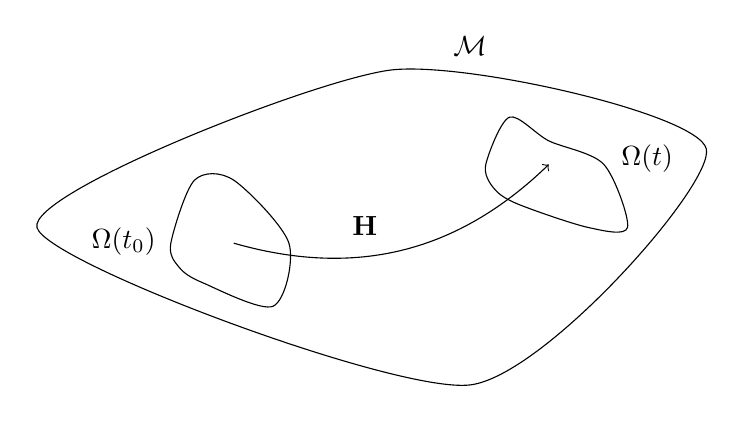
\begin{tikzpicture}
            \path[->] (0, -0.2) edge [bend right] node[left, xshift=-2mm, yshift=0.3cm] {$\mathbf H$} (4, 0.8);

            \draw[smooth cycle, tension=0.4] plot coordinates{(2,2) (-2.5,0) (3,-2) (6,1)} node at (3,2.3) {$\mathcal M$};
        
            \draw[smooth cycle] 
                plot coordinates {(0.5, -1) (0.7, -0.2) (0.0, 0.6) (-0.5, 0.6) (-0.8, -0.2) (-0.7, -0.5) (-0.4, -0.7)} 
                node [label={[label distance=-0.3cm, xshift=-1cm, yshift=0.4cm]:$\Omega (t_0)$}] {};
            \draw[smooth cycle] 
                plot coordinates {(5, 0) (4.7, 0.8) (4.0, 1.1) (3.5, 1.4) (3.2, 0.8) (3.3, 0.5) (3.6, 0.3) (4.5, 0.0)} 
                node [label={[label distance=-0.8cm, xshift=0.75cm, yshift=1.25cm]:$\Omega(t)$}] {};
        \end{tikzpicture}
        \label{fig:liou}
        \caption{The (Hamiltonian) flow of the system in which $\vol \Omega(t_0) = \vol \Omega(t)$.}
    \end{figure}

    An important corollary of the Liouville's theorem can be state about the property of the probability density distribution.
    \begin{corollary}
        The probability density distribution is constant in time. Mathematically
        \begin{equation}\label{cm:liou}
            \dv{\rho}{t} = \pdv{\rho}{t} + \{\rho, H\} = 0 ~.
        \end{equation}
    \end{corollary}
    The physical interpretation of this corollary is that particles do not appear nor disappear due to conservation of charge, mass, etc.
    \begin{proof}
        Consider the flow of a portion of phase space as it was a fluid with associated density $\rho$ and current $\mathbf J = \rho \mathbf v$. By the Liouville's theorem, it must satisfy a continuity equation 
        \begin{equation*}
            \pdv{\rho}{t} + \boldsymbol \nabla \cdot \mathbf J = 0 ~.
        \end{equation*}
        We introduce a local chart $(q^i, p_i)$ for the manifold and for the tangent space, in order to have $\mathbf v = (\dot q^i, \dot p_i)$ and $\boldsymbol \nabla = (\partial/\partial q^i, \partial/\partial p_i)$. Therefore, the continuity equation becomes
        \begin{equation*}
        \begin{aligned}
            0 & = \pdv{\rho}{t} + \boldsymbol \nabla \cdot \mathbf J \\ & = \pdv{\rho}{t} + \sum_i (\partial/\partial q^i, \partial/\partial p_i) \cdot (\dot q^i, \dot p_i) \\ & = \pdv{\rho}{t} + \sum_i ( \pdv{}{q^i} (\rho \dot q^i) + \pdv{}{p_i} (\rho \dot p_i) ) \\ & = \pdv{\rho}{t} + \sum_i ( \pdv{\rho}{q^i} \underbrace{\dot q^i}_{\pdv{H}{p_i}} + \rho \pdv{}{q^i} \underbrace{\dot q^i}_{\pdv{H}{p_i}} + \pdv{\rho}{p_i} \underbrace{\dot p_i}_{-\pdv{H}{q^i}} + \rho \pdv{}{p_i} \underbrace{\dot p_i}_{-\pdv{H}{q^i}} ) \\ & = \pdv{\rho}{t} + \sum_i ( \pdv{\rho}{q^i} \pdv{H}{p_i} + \cancel{\rho \pdvd{H}{p_i}{q^i}} - \pdv{\rho}{p_i} \pdv{H}{q^i} - \cancel{\rho \pdvd{H}{q^i}{p_i}} ) \\ & = \pdv{\rho}{t} + \sum_i ( \pdv{\rho}{q^i} \pdv{H}{p_i} - \pdv{\rho}{p_i} \pdv{H}{q^i} ) \\ & = \pdv{\rho}{t} + \{\rho, H\} ~,
        \end{aligned}
        \end{equation*}
        where we have used the Hamilton's equations~\eqref{cm:hameq}, the fact that partial derivatives commute and the definition of Poisson's brackets~\eqref{cm:poi}.
    \end{proof}

    For stationary systems, i.e. when $\pdv{\rho}{t} = 0$, the necessary condition for equilibrium is $\{\rho, H\} = 0$, which is satisfied only if 
    \begin{equation*}
        \rho(q^i, p_i) = const ~,
    \end{equation*}
    like in the microcanonical ensemble, or 
    \begin{equation}\label{cm:rh}
        \rho(q^i, p_i) = \rho(H(q^i,p_i)) ~,
    \end{equation}
    like in the canonical or in the grand canonical ensemble.

    \begin{proof}
        For the first, we have 
        \begin{equation*}
            \{\rho, H\} = \underbrace{\pdv{\rho}{q^i}}_0 \pdv{H}{p_i} - \underbrace{\pdv{\rho}{p_i}}_0 \pdv{H}{q^i} = 0 ~.
        \end{equation*}

        For the second, we have 
        \begin{equation*}
        \begin{aligned}
            \{\rho, H\} = \pdv{\rho}{q^i} \pdv{H}{p_i} - \pdv{\rho}{p_i} \pdv{H}{q^i} = \cancel{\pdv{\rho}{H} \pdv{H}{q^i} \pdv{H}{p_i}} - \cancel{\pdv{\rho}{H} \pdv{H}{p_i} \pdv{H}{q^i}} = 0 ~
        \end{aligned}
        \end{equation*}
        where we have developed the dependence of $\rho$ on $H$ by the chain rule and the fact that partial derivatives commute.
    \end{proof}

    The average value of an observable $f$ is given by the volume of the function in phase space, weighted by the probability density distribution
    \begin{equation}\label{cm:av}
        \av{f} = \int_{\mathcal M^{dN}} d\Gamma ~ \rho(q^i, ~p_i) f(q^i, ~p_i) ~,
    \end{equation}
    while the standard deviation is defined by
    \begin{equation*}
        (\Delta f)^2 = \av{f^2} - \av{f}^2 ~.
    \end{equation*}

\section{Energy foliation}

    Consider a time-independent Hamiltonian $H = H(q^i, p_i)$, which implies by the theorem~\eqref{cm:consen} that energy is conserved $E = \text{const}$. In this case, there exists $2dN - 1$ independent (local) constants of motion. However, we are interested in global integrals, which are isolating, i.e.~they admit hypersurfaces in phase space, and foliating, i.e.~they admit a foliation of phase space via surfaces of constant value, called level surfaces. The most important global foliating isolating integral is the energy, sometimes it is even the only one. Therefore, we foliate the whole phase space into $2dN - 1$-dimensional hypersurfaces $S_E$ of constant energy. See Figure~\ref{fig:fol}. Notice that the structure of the manifold does not depend on the dynamics, but hypersurfaces do, because they depend on the different Hamiltonian $H$ chosen by the dynamics. In fact, different Hamiltonian will have different foliations. Furthermore, a different choice of the initial conditions means a different hypersurface.
    \begin{figure}[h!]
        \centering
        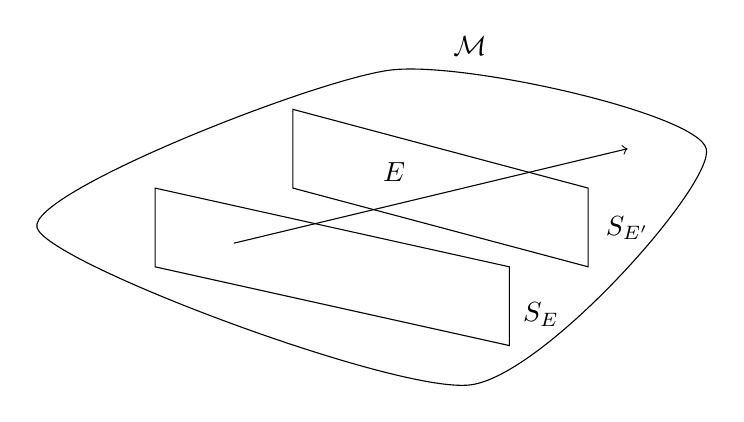
\begin{tikzpicture}
            \path[->] (0, -0.2) edge node[left, xshift=-2mm, yshift=0.3cm] {$E$} (5, 1);

            \draw[smooth cycle, tension=0.4] plot coordinates{(2,2) (-2.5,0) (3,-2) (6,1)} node at (3,2.3) {$\mathcal M$};

            \draw[smooth cycle, tension=0] 
                plot coordinates { (0.75, 0.5) (0.75, 1.5) (4.5, 0.5) (4.5, -0.5)} 
                node [label={[label distance=-0.3cm, xshift=0.5cm, yshift=0.4cm]:$S_{E'}$}] {};
            \draw[smooth cycle, tension=0] 
                plot coordinates {(-1, -0.5) (-1, 0.5) (3.5, -0.5) (3.5, -1.5)} 
                node [label={[label distance=-0.8cm, xshift=0.4cm, yshift=0.8cm]:$S_{E}$}] {};
        \end{tikzpicture}
        \label{fig:fol}
        \caption{Foliation of the phase space $\mathcal M$ by hypersurfaces $S_E$ if constant energy. In this case $E' > E$.}
    \end{figure}

    Taking advantage of this foliation structure, it is easier to compute integral in phase space. In fact, if we define the gradient of the Hamiltonian,
    \begin{equation*}
        \boldsymbol \nabla H = \pdv{H}{\boldsymbol \xi} ~,
    \end{equation*}
    which is by definition orthogonal to the energy hypersurfaces and has norm equals to 
    \begin{equation*}
        ||\boldsymbol \nabla H|| = \sqrt{\sum_i (\pdv{H}{\xi_i})^2} ~,
    \end{equation*}
    then we can decompose the phase space measure~\eqref{cm:measure} into 
    \begin{equation}\label{cm:fol}
        d \Gamma = dA dl = \underbrace{\frac{dA}{||\boldsymbol \nabla H||}}_{dS_E} \underbrace{||\boldsymbol \nabla H|| dl}_{dE} = dS_E dE ~,
    \end{equation}
    where $dA$ is the area element of the energy hypersurfaces and $dl$ is the line element orthogonal to this surface. Intuitively, we have passed from an integration of a volume of phase space $d\Gamma$ into an integration over hypersurfaces depending on the energy $dS_E$ along with an integration over energy $dE$. $dE$ is invariant, therefore $dS_E$ is an invariant area element. The volume of phase space enclosed by the energy hypersurface $S_E$ 
    \begin{equation*}
        \Sigma(E) = \{ \boldsymbol \xi \in \mathcal M \colon 0 \leq H(\xi) \leq E \} 
    \end{equation*}
    is given by 
    \begin{equation}\label{cm:vol}
        \Sigma(E) = \int_{0 \leq H \leq E} d\Gamma = \int_0^E dH \int_{S_E} dS_{H} = \int_0^E dH ~ \omega(H)
    \end{equation}
    where we have defined the density of states $\omega$ as 
    \begin{equation}\label{cm:denst}
        \omega (E) = \int_{\mathcal M^{dN}} d\Gamma ~ \delta (H- E) = \int_{S_E} dS_H = \pdv{\Sigma}{E} ~,
    \end{equation}
    where the Dirac delta $\delta (H - E)$ constrains ourselves into the hypersurface of energy $H = E$.

\section{Ergodicity}

    An important and fundamental concept in statistical mechanics is ergodicity. A physical system is said to be ergodic on an energy hypersurface of constant energy $S_E$ if and only if, in time evolution, almost\footnote{Up to a null measure set} every point $\xi^j \in S_E$ passes through every neighbourhood $U \subset S_E$. In other word, in a finite time interval $t \in (- \infty, \infty)$, the system samples every small neighbourhood of the surface and the set of trajectories is dense. Ergodicity implies that the only isolating integral is energy and there are no other conservation laws.

    Given an observable $f$, we can associate $2$ different in principle average values~\eqref{cm:av}
    \begin{enumerate}
        \item phase-space average over the energy hypersurface $S_E$, since the motion is confined inside $S_E$
            \begin{equation*}
                \av{f}_E = \frac{1}{\omega(E)} \int_{S_E} dS_H ~ f = \frac{1}{\omega(E)} \int_{\mathcal M} d \Gamma ~ \delta (H - E) f = \frac{1}{\omega(E)} \pdv{}{E} \int_{\Sigma(E)} d \Gamma ~ f ~, 
            \end{equation*}
        \item (infinite) time average, that can be experimentally obtained by observing the system over a long amount of time 
            \begin{equation*}
                \av{f}_\infty = \lim_{t \rightarrow \infty} \int_{t_0}^{t_0 + \infty} dt ~ f(q^i(t), p_i(t)) ~, 
            \end{equation*}
            which is valid for almost every initial condition and it is independent of the initial time $t_0$.
    \end{enumerate}

    Ergodicity and average values are connected by a theorem.
    \begin{theorem}
        A system is ergodic if and only if 
        \begin{equation}\label{cm:erg}
            \av{f}_E = \av{f}_\infty ~.
        \end{equation}
    \end{theorem}
    In these notes, we will consider only ergodic systems.

\section{Ensembles}

    Thermodynamics provides the completely macroscopic description of a physical system (equations of state, relations between thermodynamic quantities) once a single thermodynamic potential has been given. See Table~\ref{table:cm:1}.
    \begin{table}[h!]
        \centering
        \begin{tabular}{c | c }
            Ensemble & Thermodynamic potential \\
            \hline
            microcanonical & entropy $S$ \\ 
            canonical & Helmoltz free energy $F$ \\ 
            grand canonical & grand potential $\Omega$ \\ 
        \end{tabular}
        \caption{Ensembles with associated thermodynamic potential.}
        \label{table:cm:1}
    \end{table}
    
\chapter{Microcanonical ensemble}

\section{Microcanonical probability density distribution}

    Consider a physical system which is isolated from the environment, i.e.~it cannot exchange neither energy nor matter so that the boundary conditions are fixed $E$, $N$ and $V$. Of course, isolated systems are a bit nonphysical. Since energy is conserved and the Hamiltonian is time-independent, the trajectory of motion is restricted on the surface $S_E$ and not on all the phase space. This kind of set-up is called microcanonical ensemble and it has associated a probability density distribution, which a priori is uniform
    \begin{equation*}
        \rho_{mc}(q^i, ~p_i) = C \delta (H(q^i, p_i) - E) ~,
    \end{equation*}
    where $C$ is a normalisation constant, which can be evaluated by~\eqref{cm:norm}
    \begin{equation*}
        1 = \int_{\mathcal M^N} d\Omega ~ \rho_{mc} = \int_{\mathcal M^N} d\Omega ~ C \delta(H - E) = C \underbrace{\int_{\mathcal M^N} d\Omega ~ \delta(H - E)}_{\omega(E)} = C \omega(E) ~.
    \end{equation*}
    Hence, the microcanonical probability density distribution is
    \begin{equation}\label{mc:pdd}
        \rho_{mc}(q^i, ~p_i) = \frac{1}{\omega(E)} \delta (H(q^i, p_i) - E) ~.
    \end{equation}
    This distribution can be evaluated by the following argument: suppose that the system has not exactly energy equals to $E$, but the latter is in a range $H \in [E, E + \Delta E]$, where $\Delta E$ is an infinitesimal displacement of energy, i.e. $\Delta E \ll 1$. The volume in phase space~\eqref{cm:vol} becomes 
    \begin{equation*}
        \Gamma (E) = \integ{E}{E+\Delta E}{E'} \omega(E') \simeq \omega(E) \Delta E = \pdv{\Sigma(E)}{E} \Delta E ~.
    \end{equation*}
    Consequently, the distribution becomes 
    \begin{equation*}
        \rho_{mc}(q^i, p_i) = \begin{cases}
            \frac{1}{\Gamma(E)} & H \in [E, E + \Delta E] \\
            0 & otherwise
        \end{cases}
    \end{equation*}
    Therefore, in the limit for which $\Delta E \rightarrow 0$, we can find exactly~\eqref{mc:pdd}, up to the normalisation constant.

    Let $f(q^i, p_i)$ be an observable, then its microcanonical average (or equivalenty is energy hypersurface average) is 
    \begin{equation}\label{mc:av}
        \avp{f(q^i, p_i)}{mc} = \int_{\mathcal M} d\Omega ~ \rho_{mc} f = \int_{\mathcal M} d\Omega ~ \frac{1}{\omega(E)} \delta (H - E) f = \frac{1}{\omega(E)} \int_{S_E} dS_E ~ f = \avp{f}{E} ~.
    \end{equation}

\section{Entropy as microcanonical potential}

    A local chart with coordinates $(E, V, N)$ is suitable for entropy~\eqref{td:coord:s}. Hence, we need to find an expression for entropy. The first guess is to define the microcanonical entropy $S_{mc}$ as 
    \begin{equation}\label{mc:s}
        S_{mc} (E, V, N) = k_B \ln \Gamma(E) ~,
    \end{equation}
    which, in the thermodynamic limit, it is equivalent to
    \begin{equation*}
        s_{mc} = \lim_{td} \frac{S_{mc}}{N} = k_B \lim_{td} \frac{\log \omega(E)}{N} = \underbrace{k_B \lim_{td} \frac{\log \Sigma(E)}{N}}_{H \in [0, E]} = \underbrace{k_B \lim_{td} \frac{\log \Gamma(E)}{N}}_{H \in [E, E + \Delta E]} ~.
    \end{equation*}
    The logarithm is justified by the fact that the volume of a $N$-particle phase space is $(W_1)^N$, where $W_1$ is the volume of a single particle phase space. According to the properties of the logarithm, in this way, entropy becomes extensive.

    Now, we need to prove that~\eqref{mc:s} is indeed the thermodynamic entropy. The first property that it must fulfill is additivity: given $2$ subsystems $A$ and $B$, the total entropy is the sum of the $2$ separately subsystems entropy
    \begin{equation*}
        s_{mc}^{tot} = s_{mc}^{(1)} + s_{mc}^{(2)} ~.
    \end{equation*}
    \begin{proof}
        Consider two isolated subsystems $A$ and $B$ in contact at thermal equilibrium with the same temperature $T = T_1 = T_2$ but whatsoever volume $V_1$ and $V_2$ and energies $E_1$ and $E_2$. The total system is isolated and it can be treated as a microcanonical ensemble. The entropy of the subsystems will be respectively 
        \begin{equation*}
            S_1 = k_B \ln \Gamma_1(E_1) ~, \quad S_2 = k_B \ln \Gamma_2 (E_2) ~.
        \end{equation*}
        where $\Gamma_1 (E_1) \simeq \omega_1 (E_1) \Delta E_1$ and $\Gamma_2 (E_2) \simeq \omega_2 (E_2) \Delta E_2$. The total energy is $E = E_1 + E_2 + E_{surface}$ but, in the thermodynamic limit, the energy exchanged by the surface is a subleading term ($E_1$ and $E_2$ go as $L^3$ whereas $E_{surface}$ goes as $L^2$) and then it can be neglected. Therefore, the total energy becomes $E = E_1 + E_2$. The joint density of states is 
        \begin{equation*}
        \begin{aligned}
            \omega(E) & = \int_{\mathcal M^N} \underbrace{d\Gamma_1}_{dE_1 dS_{E_1}} ~ \underbrace{d\Gamma_2}_{dE_2 dS_{E_2}} ~ \delta(H - E) \\ & = \int dE_1 \int dS_{E_1} \int dE_2 \int dS_{E_2} ~ \delta (E - E_1 - E_2) \\ & = \int dE_1 \int dE_2 ~ \omega_1(E_1) \omega_2(E_2) \delta (E - E_1 - E_2) \\ & = \int_0^E dE_1 ~ \omega_1(E_1) \omega_2(E_2 = E - E_1) ~.
        \end{aligned}
        \end{equation*}
        Notice that the integrand is a positive function and it has a maximum in $E^*_1 \in [0, E]$. Hence, we can find an upper bound for the integral, which is
        \begin{equation}\label{proof1}
        \begin{aligned}
            \integ{0}{E}{E_1} \omega_1(E_1) \omega_2(E_2 = E - E_1) & \leq \omega_1(E^*_1) \omega_2(E^*_2 = E - E^*_1) \underbrace{\int_0^E dE_1}_E \\ & = \omega_1(E^*_1) \omega_2(E^*_2 = E - E^*_1) E ~.
        \end{aligned}
        \end{equation}
        On the other hand, it is always possible to find a value for a small enough $\Delta E$ in order to have 
        \begin{equation} \label{proof2}
            \omega_1(E^*_1) \omega_2(E^*_2 = E - E^*_1) \Delta E \leq \omega(E) ~.
        \end{equation}
        Putting together~\eqref{proof1} and~\eqref{proof2}, we obtain, after a series of manipulations
        \begin{equation*}
            \Delta E \omega_1(E^*_1) \omega_2(E^*_2) \leq \omega(E) \leq \omega_1(E^*_1) \omega_2(E^*_2) E ~,
        \end{equation*}
        \begin{equation*}
            \underbrace{\omega_1(E^*_1) \Delta E}_{\Gamma_1 (E^*_1)} \underbrace{\omega_2(E^*_2) \Delta E}_{\Gamma_2 (E^*_2)} \leq \underbrace{\omega(E) \Delta E}_{\Gamma(E)} \leq \frac{E}{\Delta E} \underbrace{\omega_1(E^*_1) \Delta E}_{\Gamma_1 (E^*_1)} \underbrace{\omega_2(E^*_2) \Delta E}_{\Gamma_2 (E^*_2)} ~,
        \end{equation*}
        \begin{equation*}
            \Gamma_1(E^*_1) \Gamma(E^*_2) \leq \Gamma(E) \leq \frac{E}{\Delta E}\Gamma(E^*_1) \Gamma(E^*_2) ~.
        \end{equation*}
        Now, we can take the logarithm, since it is a monotonic function, after another series of manipulations, we obtain
        \begin{equation*}
            \log ( \Gamma_1(E^*_1) \Gamma(E^*_2) ) \leq \log \Gamma(E) \leq \log ( \frac{E}{\Delta E}\Gamma(E^*_1) \Gamma(E^*_2) ) ~,
        \end{equation*}
        \begin{equation*}
            k_B \log \Big ( \Gamma_1(E^*_1) \Gamma(E^*_2) \Big ) \leq k_B \log \Gamma(E) \leq k_B \log \Big ( \frac{E}{\Delta E}\Gamma(E^*_1) \Gamma(E^*_2) \Big ) ~,
        \end{equation*}
        \begin{equation*}
        \begin{aligned}
            k_B \log \Gamma_1(E^*_1) + k_B \log \Gamma(E^*_2) & \leq k_B \log \Gamma(E) \\ & \leq k_B \log \frac{E}{\Delta E} + k_B \log \Gamma(E^*_1) + k_B \log \Gamma(E^*_2) ~,
        \end{aligned}
        \end{equation*}
        \begin{equation*}
        \begin{aligned}
            \frac{k_B \log \Gamma_1(E^*_1) + k_B \log \Gamma(E^*_2)}{N} & \leq \frac{k_B \log \Gamma(E)}{N} \\ & \leq \frac{k_B \log \Gamma(E^*_1) + k_B \log \Gamma(E^*_2)}{N} + \frac{k_B \log \frac{E}{\Delta E}}{N} ~.
        \end{aligned}
        \end{equation*}
        Finally, we take the thermodynamic limit, noticing that the last term vanishes, since $E$ goes like $N$ and $\lim_{N \rightarrow \infty} \frac{1}{N} \log N = 0$
        \begin{equation*}
        \begin{aligned}
            \underbrace{\lim_{TD} \frac{k_B \log \Gamma_1(E^*_1)}{N}}_{s_{mc}^{(1)}} + \underbrace{\lim_{TD} \frac{k_B \log \Gamma(E^*_2)}{N}}_{s_{mc}^{(2)}} & \leq \underbrace{\lim_{TD} \frac{k_B \log \Gamma(E)}{N}}_{s_{mc}} \\ & \leq \underbrace{\lim_{TD} \frac{k_B \log \Gamma_1(E^*_1)}{N}}_{s_{mc}^{(1)}} + \underbrace{\lim_{TD} \frac{k_B \log \Gamma(E^*_2)}{N}}_{s_{mc}^{(2)}} ~,
        \end{aligned}
        \end{equation*}
        hence
        \begin{equation}\label{proof3}
            s_{mc}(E) = s_{mc}^{(1)} (E_1^*) + s_{mc}^{(2)} (E_2^*) ~.
        \end{equation}
    \end{proof}

    From~\eqref{proof3}, we can also deduce $2$ properties that entropy fulfills: for isolated system, spontaneous processes leads to an increase in entropy, which is verified because spontaneous processes leads also to an increase in phase space volume; at equilibrium, entropy is maximum, which is verified by the asterisks. Furthermore, in the thermodynamic limit, microcanonical entropy coincides with thermodynamic entropy
    \begin{equation*}
        s_{mc} = s_{td} ~.
    \end{equation*}
    \begin{proof}
        Since entropy is maximum at equilibrium, also $\Gamma_1(E_1) \Gamma_2(E_2)$ is so and it has null variation
        \begin{equation*}
        \begin{aligned}
            0 & = \delta (\Gamma_1(E^*_1) \Gamma_2(E^*_2 = E - E^*_1)) \\ & = \delta \Gamma_1(E^*_1) \Gamma_2 (E^*_2) + \Gamma_1(E^*_1) \delta \Gamma_2 (E^*_2) \\ & = \pdv{\Gamma_1}{E_1} \Big\vert_{E^*_1} \delta E_1 \Gamma_2 (E^*_2) + \Gamma_1(E^*_1) \pdv{\Gamma_2}{E_2} \Big\vert_{E^*_2} \delta E_2 ~,
        \end{aligned}
        \end{equation*}
        where we have used Leibniz rule and we have exploited the dependence on energy.

        Since $E = \text{const}$, it has a null variation $0 = \delta E = \delta E_1 + \delta E_2$ and 
        \begin{equation}\label{proof4}
            \delta E_2 = - \delta E_1 ~.
        \end{equation} 
        Hence, with a series of manipulations, we obtain
        \begin{equation*}
            0 = \pdv{\Gamma_1}{E_1} \Big\vert_{E^*_1} \delta E_1 \Gamma_2 (E^*_2) - \Gamma_1(E^*_1) \pdv{\Gamma_2}{E_2} \Big\vert_{E^*_2} \delta E_1  ~,
        \end{equation*}
        \begin{equation*}
            0 = \pdv{\Gamma_1}{E_1} \Big\vert_{E^*_1} \Gamma_2 (E^*_2) - \Gamma_1(E^*_1) \pdv{\Gamma_2}{E_2} \Big\vert_{E^*_2}  ~,
        \end{equation*}
        \begin{equation*}
            \pdv{\Gamma_1}{E_1} \Big\vert_{E^*_1} \Gamma_2 (E^*_2) = \Gamma_1(E^*_1) \pdv{\Gamma_2}{E_2} \Big\vert_{E^*_2} ~,
        \end{equation*}
        \begin{equation*}
            \frac{1}{\Gamma_1 (E^*_1)} \pdv{\Gamma_1}{E_1} \Big\vert_{E^*_1} = \frac{1}{\Gamma_2 (E^*_2)} \pdv{\Gamma_2}{E_2} \Big\vert_{E^*_2} ~,
        \end{equation*}
        \begin{equation*}
            \pdv{\log \Gamma_1}{E_1} \Big\vert_{E^*_1} = \pdv{\log \Gamma_2}{E_2} \Big\vert_{E^*_2} ~.
        \end{equation*}
        This is a relation valid for all systems at equilibrium, which is the $0$th law of thermodynamic. Finally, we use the first thermodynamic relation in~\eqref{td:es:s} to have
        \begin{equation*}
            S_{mc} (E) = S_{td} (E) \times const
        \end{equation*}
        where the constant can be chosen the Boltzmann constant, in order to have $k_B$ in the same unit of energy over temperature.
    \end{proof}

    The universal Boltzmann's formula is 
    \begin{equation}\label{mc:unibol}
        s_{mc} = s_{td} = k_B \log \omega(E) = - k_B \avp{\log \rho_{mc}}{mc} ~.
    \end{equation}
    \begin{proof}
        In fact, using~\eqref{mc:av} and the properties of logarithms, 
        \begin{equation*}
        \begin{aligned}
            \avp{\log \rho_{mc}}{mc} & = \int d\Gamma ~ \rho_{mc} \log \rho_{mc} \\ & = \int d\Gamma ~ \frac{1}{\omega(E)} \delta (H - E) \log \Big ( \frac{1}{\omega(E)} \delta (H - E) \Big) \\ & = \int dS_E ~ \frac{1}{\omega(E)} \log \frac{1}{\omega(E)} \\ & = - \frac{1}{\omega(E)} \log \omega(E) \underbrace{\int dS_E }_{\omega(E)} \\ & = - \log \omega (E) ~.
        \end{aligned}
        \end{equation*}
    \end{proof}

\chapter{Canonical ensemble}

\section{Canonical probability density distribution}

    Consider a physical system which can exchange energy with the environment but matter, so that the boundary conditions are fixed $T$, $N$ and $V$. Notice that temperature has substituted energy. Physically, it can be thought as the system is immersed in a bigger reservoir with $N_S \ll N_E$ and $V_S \ll V_E$ but at equilibrium with the same temperature $T_S = T_E = T$. See Figure~\ref{fig:c}. 

    \begin{figure}[h!]
        \centering
        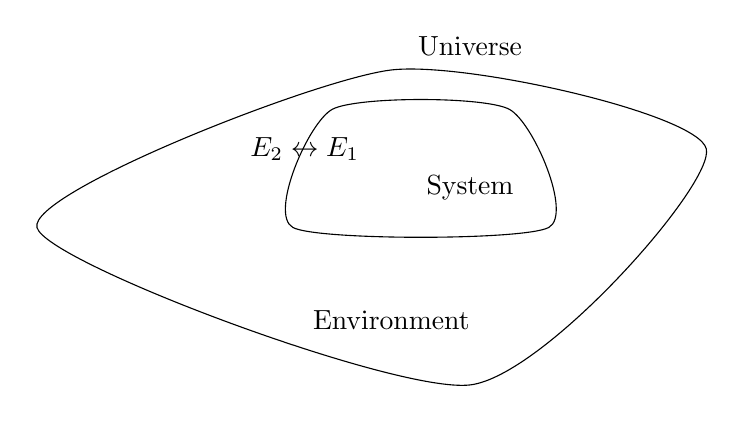
\begin{tikzpicture}
            \draw[smooth cycle, tension=0.4] plot coordinates{(2,2) (-2.5,0) (3,-2) (6,1)} node at (3,2.3) {Universe};

            \draw[smooth cycle, tension=0.4] 
                plot coordinates { (0.75, 0) (1.25, 1.5) (3.5, 1.5) (4, 0)} 
                node [label={[label distance=-0.3cm, xshift=-1cm, yshift=0.4cm]:System}] {}
                node [label={[label distance=-0.3cm, xshift=-2cm, yshift=-1.25cm]:Environment}] {};

            \node[] at (0.9, 1) {$E_2 \leftrightarrow E_1$};
        \end{tikzpicture}
        \label{fig:c}
        \caption{Pictorial representation of canonical ensemble.}
    \end{figure}

    Globally, energy is conserved and the universe, composed by the union of the system and the environment, can be considered isolated and, therefore, a microcanonical ensemble. This kind of set-up is called canonical ensemble and it has associated a probability density distribution 
    \begin{equation}\label{c:pdd}
        \rho_c (q^i, p_i) = \frac{1}{Z_N} \exp (-\beta H(q^i, p_i)) ~,
    \end{equation}
    where $\beta$ is 
    \begin{equation*}
        \beta = \frac{1}{k_B T}
    \end{equation*}
    and $Z_N$ is the partition function 
    \begin{equation}\label{c:z}
        Z_N[V, T] = \int_{\mathcal M^N} d\Omega ~\exp (-\beta H(q^i, p_i)) ~,
    \end{equation}
    which depends on the temperature through $\beta$ and volume and temperature due to the integration domain $\mathcal M^N = V \otimes \mathbb R^d$. Notice that the probability is a function of the Hamiltonian, like Liouville's theorem said~\eqref{cm:rh}.
    \begin{proof}
        Consider the universe as a microcanonical ensemble, with associated probability density distribution as
        \begin{equation*}
            \rho_{mc} (q_i^{(1)}, p_i^{(1)}, q_i^{(2)}, p_i^{(2)}) = \frac{1}{\omega(E)} \delta (H (q_i^{(1)}, p_i^{(1)}, q_i^{(2)}, p_i^{(2)}) - E) ~,
        \end{equation*}
        where $1$ is the system, $2$ is the environment and the total Hamiltonian is 
        \begin{equation*}
            H (q_i^{(1)}, p_i^{(1)}, q_i^{(2)}, p_i^{(2)}) = H_1 (q_i^{(1)}, p_i^{(1)}) + H_2 (q_i^{(2)}, p_i^{(2)}) ~.
        \end{equation*}
        To find the probability density distribution for only the degrees of freedom associated to the system, we have to integrate over the degrees of freedom of the environment to wash them out
        \begin{equation*}
            \rho^{(1)} = \int d\Omega_2 ~ \rho_{mc} = \int d\Omega_2 ~ \frac{1}{\omega(E)} \delta(H - E) = \frac{1}{\omega(E)} \underbrace{\int dS_{E_2}}_{\omega(E_2)} = \frac{1}{\omega(E)} \omega(E_2 = E - E_1) ~.
        \end{equation*}
        Notice that this distribution is normalised, since 
        \begin{equation*}
        \begin{aligned}
            \int d\Omega_1 ~ \rho^{(1)} & = \frac{1}{\omega(E)} \int d\Omega_1 \omega(E_2 = E - E_1) \\ & = \frac{1}{\omega(E)} \int_0^E dE_1 ~ \underbrace{\int_{S_{E_1}} dS_{H_1}}_{\omega(E-1)} \omega(E_2 = E - E_1) \\ & = \frac{1}{\omega(E)} \underbrace{\int_0^E dE_1 \omega(E_1) \omega(E_2 = E - E_1) }_{\omega(E)} = 1 ~,
        \end{aligned}
        \end{equation*}
        where the last expression follows from $E = E_1 + E_2$, $d\Omega = d\Omega_1 d\Omega_2$ and 
        \begin{equation*}
        \begin{aligned}
            \omega(E) & = \int d\Omega \delta(H - E) \\ & = \int d\Omega_1 d\Omega_2 \delta(E - E_1 - E_2) \\ & = \int dE_1 \int dE_2 \underbrace{\int_{S_{E_1}} dS_{H_1}}_{\omega(E_1)} \underbrace{\int_{S_{E_2}} dS_{H_2}}_{\omega(E_2)} \delta(E - E_1 - E_2) \\ & = \int dE_1 \int dE_2 \omega(E_1) \omega(E_2) \delta(E - E_1 - E_2) \\ & = \int dE_1 \omega(E_1) \omega(E_2 = E - E_1) ~.
        \end{aligned}
        \end{equation*}
        In order to compute $\omega(E_2)$, we introduce the entropy 
        \begin{equation*}
            S_2 (E_2) = k_B \ln \omega_2 (E_2) ~.
        \end{equation*}
        For the considerations made in the microcanonical, at equilibrium entropy is at maximum but if we make small variation $\delta E_1$ to $E_1$, in order to preserve equilibrium, the entropy get Taylor expanded around $E$ as
        \begin{equation*}
            k_B \ln \omega_2 (E_2) = S_2 (E_2) \simeq S_2(E) + \underbrace{\delta E_2}_{- \delta E_1 \simeq - E_1} \underbrace{\pdv{S_2}{E_2} \Big \vert_{E = E_2}}_{\frac{1}{T}} = S_2 (E) - E_1 \frac{1}{T} ~,
        \end{equation*} 
        where we have used~\eqref{proof4} and the first thermodynamic relation in~\eqref{td:es:s}. Hence, the density of states of the system is
        \begin{equation*}
            \omega_2 (E_2) = \exp (\frac{S_2 (E)}{k_B} - E_1 \frac{1}{k_B T}) = \exp (\frac{S_2 (E)}{k_B}) \exp (- \frac{E_1}{k_B T}) ~.
        \end{equation*}
        Finally, putting together and dropping the indices, we obtain
        \begin{equation}
            \rho_c = \frac{\omega_2 (E_2)}{\omega(E)} = \underbrace{\frac{1}{\omega(E)} \exp (\frac{S_{mc}(E)}{k_B})}_C \exp (- \frac{E_1}{k_B T}) = C \exp (- \frac{E_1}{k_B T}) ~,
        \end{equation}
        where $C$ is a normalisation constant, which can be evaluated by~\eqref{cm:norm}
        \begin{equation*}
            1 = \int_{\mathcal M^N} d\Omega \rho = \int_{\mathcal M^N} d\Omega ~ C \exp (- \frac{E_1}{k_B T}) = C \int_{\mathcal M^N} d\Omega ~ \exp (- \frac{E_1}{k_B T}) ~. 
        \end{equation*}
    \end{proof}

    The partition function can also be written as 
    \begin{equation*}
        Z_N[T, V] = \int_{0}^{\infty} dE~ \omega(E) \exp (-\beta E) ~.
    \end{equation*}
    \begin{proof}
        In fact, using~\eqref{cm:fol} we have
        \begin{equation*}
            Z_N = \int_{\mathcal M^N} d\Omega \exp (- \beta H) = \integ{0}{\infty}{E} \underbrace{\int dS_E}_{\omega(E)} ~ \exp (-\beta H) = \integ{0}{\infty}{E} \omega(E) \exp (-\beta E) ~.
        \end{equation*}
    \end{proof}

    Now, it is important to distinguish $2$ different type of particles: indistinguishable and distinguishable particles. Particles are called indistinguishable if they cannot be distinguished if compared with others and they are distinguishable otherwise. In principle, in classical physics, there are no indistinguishable particles, because even if they all have the same mass, charge, spin, etc, we could always follow their trajectory. Therefore, indistinguishable particles arise only in quantum mechanics, when the uncertainty principle is introduce and the trajectory distinction cannot be made anymore. To take into account this property, we introduce a new term $\zeta_N$, defined as 
    \begin{equation*}
        \zeta_N = \begin{cases}
            1 & \textnormal{distinguishable} \\
            N! & \textnormal{indistinguishable}
        \end{cases} ~.
    \end{equation*}
    Hence, the partition function becomes
    \begin{equation*}
        Z_N = \int \frac{\prod_{i=1}^N d^d q^i d^d p^i}{h^{dN} \zeta_N} ~ \exp (- \beta H) = \int \frac{d\Omega_N}{\zeta_N} ~ \exp (- \beta H) ~,
    \end{equation*}
    where we have redefined the phase space measure 
    \begin{equation*}
        d\Omega_N = \frac{\prod_{i=1}^N d^d q^i d^d p_i}{h^{dN}} ~.
    \end{equation*}

    For distinguishable particles, e.g.~particles of $n$ different species with energy $H = \sum_{i = 1}^{n} H_i$ and numbers $N = \sum_{i=1}^n N_i$, the total partition function is the multiplication of single species partition functions
    \begin{equation*}
        Z_N = \prod_{i = 1}^{n} Z_{N_i} ~.
    \end{equation*}
    \begin{proof}
        In fact, 
        \begin{equation*}
        \begin{aligned}
            Z_N & = \int_{\mathcal M = \mathcal M^{(1)}\times \ldots \times \mathcal M^{(n)}} d\Omega ~\exp (-\beta H) \\ & = \int_{\mathcal M = \mathcal M^{(1)}\times \ldots \times \mathcal M^{(n)}} \prod_{i = 1}^{n} d\Omega_i \ldots d\Omega_n ~ \exp(-\beta \sum_{i = 1}^{N} H_i) \\ & = \prod_{i = 1}^{n} \int_{\mathcal M^{(i)}} d\Omega_i ~ \exp(- \beta H_i) = \prod_{i = 1}^{n} Z_{N_i} ~.
        \end{aligned}
        \end{equation*}
    \end{proof}

    \begin{example}
        If we have only $2$ types of particles, the total partition function is 
        \begin{equation*}
            Z_N = Z_{N_1} Z_{N_2} ~.
        \end{equation*}
    \end{example}

    Consequently, if all particles are of the same species, and therefore identical, the total partition function is 
    \begin{equation*}
        Z_N = (Z_1)^N ~,
    \end{equation*}
    where $Z_1$ the single-particle partition function. 
    If we take into consideration also indistinguishability, for different species, the canonical partition function becomes 
    \begin{equation*}
        Z_N = \frac{1}{\zeta_N} \prod_{i=1}^{n} Z_{N_i} ~,
    \end{equation*}
    whereas for same species particles, it becomes
    \begin{equation*}
        Z_N = \frac{(Z_1)^N}{\zeta_N} ~.
    \end{equation*}
    
    Let $f(q^i, p_i)$ be an observable, then its canonical average is 
    \begin{equation*}\label{c:av}
        \av{f(q^i, p_i)}_{c} = \int_{\mathcal M} d\Omega ~ \rho_{c} f = \int_{\mathcal M} d\Omega ~ \frac{\exp (-\beta H)}{Z_N} f ~.
    \end{equation*}

\section{Helmoltz free energy as canonical potential}

    A local chart with coordinates $(T, V, N)$ is suitable for Helmoltz free energy~\eqref{td:coord:f}. Hence, we need to find an expression for this thermodynamic potential.
    The first guess is to define the canonical Helmoltz free energy as 
    \begin{equation}\label{c:zf}
        Z_N [V, T] = \exp(-\beta F[T, V, N]) ~,
    \end{equation}
    or, equivalently,
    \begin{equation}\label{c:f}
        F[T, V, N] = -\frac{1}{\beta} \ln Z_N ~.
    \end{equation}
    Furthermore, the canonical internal energy is 
    \begin{equation}\label{c:e}
        E = \avp{H}{c} = \int d\Omega \frac{\exp(-\beta (H))}{Z_N} H ~.
    \end{equation}

    \begin{proof}
        By normalisation condition, we have
        \begin{equation*}
            1 = \int d\Omega \frac{\exp(-\beta H)}{Z_N} = \int d\Omega \frac{\exp(-\beta H)}{\exp(-\beta F)} = \int d\Omega \exp (- \beta (H - F)) ~.
        \end{equation*}
        Now, since $F$ depends on the temperature $F(T)$ or $F(\beta)$, it is possible to derive it with respect to $\beta$, where the left handed side is null because it is the derivative of a constant $1$, and we obtain
        \begin{equation*}
        \begin{aligned}
            0 & = \pdv{}{\beta} \Big ( \int d\Omega \exp (- \beta (H - F)) \Big) \\ & = \int d\Omega \exp (-\beta (H - F)) \Big (-(H - F) + \beta \pdv{F}{\beta}) \\ & = - \underbrace{\int d\Omega \frac{\exp(-\beta H)}{Z_N} H}_{E} + F \underbrace{\int d\Omega \frac{\exp(-\beta H)}{Z_N}}_{1} + \beta \pdv{F}{\beta} \underbrace{\int d\Omega \frac{\exp(-\beta H)}{Z_N}}_{1} \\ & = - E + F + \beta \pdv{F}{\beta} ~.
        \end{aligned}
        \end{equation*}
        Hence, using the first expression of~\eqref{td:es:f}, we find
        \begin{equation*}
            F = E - \beta \pdv{F}{\beta} = E + T \pdv{F}{T} = E - TS ~,
        \end{equation*}
        where in the first step we have used 
        \begin{equation*}
            \beta \pdv{}{\beta} = \frac{1}{k_B} T \pdv{T}{\beta} \pdv{}{T} = \frac{1}{k_B T} (\pdv{}{T} \frac{1}{k_B T})^{-1} \pdv{}{T} = - \frac{1}{T} T^2 \pdv{}{T} = - T \pdv{}{T} ~.
        \end{equation*}
        This result shows explicitly that $F$ is indeed the Helmotz free energy~\eqref{td:def:f}.
    \end{proof}
    Notice that canonical entropy can be written as 
    \begin{equation} \label{c:s}
        S_c = \frac{E - F}{T} ~.
    \end{equation}
    
    An useful expression for the internal energy is
    \begin{equation}\label{c:e2}
        E = - \pdv{}{\beta} \ln Z_N ~,
    \end{equation}
    \begin{proof}
        Using~\eqref{c:e},
        \begin{equation*}
        \begin{aligned}
            E & = \int d\Omega \frac{\exp(-\beta H)}{Z_N} H = - \frac{1}{Z_N} \pdv{}{\beta} \int d\Omega \exp (-\beta H) \\ & = - \frac{1}{Z_N} \pdv{Z_N}{\beta} = - \pdv{}{\beta} \ln Z_N ~,
        \end{aligned}
        \end{equation*}
        where we have used the trick to extract the derivative with respect to $\beta$.
    \end{proof}

    The universal Boltzmann's formula is valid also in this ensemble
    \begin{equation*}
        S_c = -k_B \avp{\ln \rho_c}{c}  ~.
    \end{equation*}
    \begin{proof}
        In fact, using~\eqref{c:e},~\eqref{c:s} and~\eqref{c:f}
        \begin{equation*}
        \begin{aligned}
            -k_B \avp{\ln \rho_c}{c} & = -k_B \int d\Omega \rho_c \ln \rho_c \\ & = -k_B \int d\Omega \rho_c \ln \frac{\exp(-\beta H)}{Z_N} \\ & = -k_B \int d\Omega \rho_c \ln \exp(-\beta H) - k_B \int d\Omega \rho_c \ln Z_N \\ & = k_B  \beta \underbrace{\int d\Omega \rho_c H }_E - k_B \underbrace{\ln Z_N}_{\beta F} \underbrace{\int d\Omega \rho_c}_{1} \\ & = \frac{E - F}{T} = S_c ~.
        \end{aligned}
        \end{equation*}
    \end{proof}

\section{Equipartition theorem}

    An important theorem, that can be proved in the canonical ensemble, is the famous equipartition theorem. In this section, we will proved a generalised version of it.

    \begin{theorem}[Generalised equipartition theorem]
        Let $\xi \in [a,b]$ be a sympletic coordinate. Let $\xi_j$ with $j \neq 1$ be all the other ones. Suppose also 
        \begin{equation}\label{equi:cond}
            \int \prod_{j \neq 1} d \xi_j [\xi_1 \exp(-\beta H)]_a^b = 0 ~.
        \end{equation}
        Then 
        \begin{equation}\label{equi:thm}
            \avp{\xi_1 \pdv{H}{\xi_1}}{c} = k_B T ~.
        \end{equation}
    \end{theorem}

    \begin{proof}
        By normalisation condition, we have
        \begin{equation*}
            1 = \int d\Omega ~ \frac{\exp(-\beta H)}{Z_N} = \frac{1}{Z_N} \int d\xi_1 \prod_{j \neq 1} d \xi_j ~ \exp(-\beta H) ~,
        \end{equation*}
        where we have omitted dimensional and indistinguishability factors for convenience.
        Now, using a differential relation, which is equivalent to an intergation by parts,
        \begin{equation*}
            d(\xi_1 \exp(-\beta H)) = d\xi_1 \exp(-\beta H) + \xi \exp(-\beta H) (-\beta) \pdv{H}{\xi_1} d\xi_1  ~,
        \end{equation*}
        we invert it 
        \begin{equation*}
            d\xi_1 \exp(-\beta H) = d(\xi_1 \exp(-\beta H)) + \beta \xi \exp(-\beta H) \pdv{H}{\xi_1} d\xi_1
        \end{equation*}
        and we insert it to find
        \begin{equation*}
        \begin{aligned}        
            1 & = \frac{1}{Z_N} \int (\prod_{j \neq 1} d \xi_j) (d(\xi_1 \exp(-\beta H)) + \beta \xi \exp(-\beta H) \pdv{H}{\xi_1} d\xi_1) \\ & = \frac{1}{Z_N} \underbrace{\prod_{j \neq 1} d \xi_j [\xi_1 \exp(-\beta H)]_a^b}_{0} + \frac{\beta}{Z_N} \int \underbrace{\prod_{j \neq 1} d \xi_j d\xi_1}_{d\Omega} ~ \xi_1 \pdv{H}{\xi_1} \exp (-\beta H) \\ & = \beta \int d\Omega ~ \xi_1 \pdv{H}{\xi_1} \frac{\exp (- \beta H)}{Z_N} \\ & = \beta \avp{\xi_1 \pdv{H}{\xi_1}}{c}
        \end{aligned}
        \end{equation*}
        where we have used the hypothesis~\eqref{equi:cond}.
        Hence
        \begin{equation*}
            \avp{\xi_1 \pdv{H}{\xi_1}}{c} = \frac{1}{\beta} = k_B T ~.
        \end{equation*}
    \end{proof}

    One may wonder which are the physical systems that satisfy the strange condition~\eqref{equi:cond}. Examples are systems with Hamiltonian composed by a quadratic momentum (with $a = -\infty$ and $b = \infty$) or a confining potential which go to infinity on the extremes $a$ and $b$. For the first case, we have $p \in (-\infty, \infty)$, $H = H(p^2)$ and
    \begin{equation*}
        p \exp(-\beta p^2) \Big \vert_{-\infty}^\infty = 0 ~,
    \end{equation*}
    whereas for the second case, we have $q \in [a, b]$, $V = V(q)$ such that $V(a) = V(b) = \infty$ and 
    \begin{equation*}
        q \exp(-\beta V(q)) \Big \vert_a^b = 0 ~.
    \end{equation*}

    \begin{corollary}[Equipartition theorem]
        If $\xi_1$ appears quadratically in $H$, then its contribution to $E$ is $\frac{1}{2} k_B T$.
    \end{corollary}

    \begin{proof}
        Consider $H = A \xi_1^2 + B \xi_j^2$ with $j \neq 1$, then by the means of the previous theorem, we obtain 
        \begin{equation*}
            \avp{\xi_1 \pdv{H}{\xi_1}}{c} = \avp{\xi 2 A \xi_1}{c} = k_B T ~,
        \end{equation*}
        hence
        \begin{equation*}
            \avp{A \xi_1^2}{c} = \frac{1}{2} k_B T ~.
        \end{equation*}
    \end{proof}

    \begin{example}
        Consider a perfect gas, composed by $N$ particles in $3$ dimension, with Hamiltonian $H = \sum_{i=1}^{3N} \frac{p_i^2}{2m}$. Applying the equipartition theorem, since there are $3N$ quadratic momenta terms, the energy is $E = \frac{3}{2} N k_B T$.
    \end{example}
    \begin{example}
        Consider a system composed by $N$ uncoupled harmonic oscillators of masses $m_i$ and frequencies $\omega_i$ in $3$ dimension with Hamiltonian $H = \sum_{i=1}^{3N} \frac{p_i^2}{2m_i} + \frac{m_i \omega_i q_i^2}{2}$. Applying the equipartition theorem, since there are $3N$ quadratic momenta terms and $3N$ quadratic coordinates terms, the energy is $E = 3 N k_B T$, known as the Dulong-Petit laws for the specific heat at constant volume $C_V = 3 N k_B$.
    \end{example}

\chapter{Grand canonical ensemble}

\section{Grand canonical probability density distribution}

    Consider a physical system which can exchange both energy and matter with the environment, so that the boundary conditions are fixed $T$, $V$ and $\mu$. Notice that chemical potential has substituted number of particle. Physically, it can be thought as the system is immersed in a bigger reservoir with $N_S \ll N_E$ and $V_S \ll V_E$ but at equilibrium with the same temperature $T_S = T_E = T$. See Figure~\ref{fig:gc}. 

    \begin{figure}[h!]
        \centering
        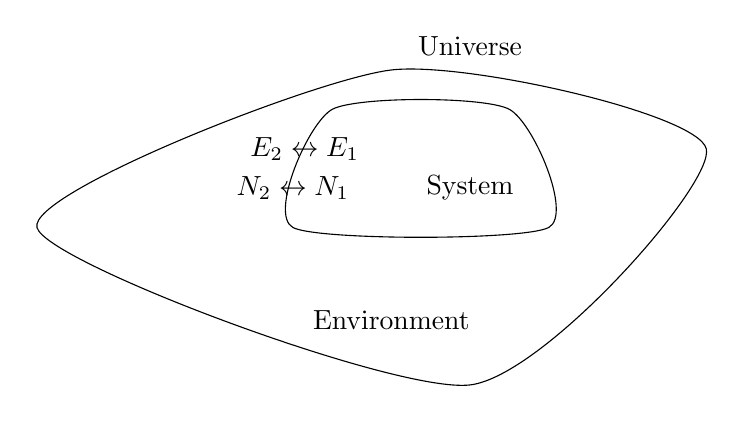
\begin{tikzpicture}
            \draw[smooth cycle, tension=0.4] plot coordinates{(2,2) (-2.5,0) (3,-2) (6,1)} node at (3,2.3) {Universe};

            \draw[smooth cycle, tension=0.4] 
                plot coordinates { (0.75, 0) (1.25, 1.5) (3.5, 1.5) (4, 0)} 
                node [label={[label distance=-0.3cm, xshift=-1cm, yshift=0.4cm]:System}] {}
                node [label={[label distance=-0.3cm, xshift=-2cm, yshift=-1.25cm]:Environment}] {};

            \node[] at (0.9, 1) {$E_2 \leftrightarrow E_1$};
            \node[] at (0.75, 0.5) {$N_2 \leftrightarrow N_1$};
        \end{tikzpicture}
        \label{fig:gc}
        \caption{Pictorial representation of grand canonical ensemble.}
    \end{figure}
    
    Globally, number of particles is conserved and the universe, composed by the union of the system and the environment, can be considered a canonical ensemble. In fact we suppose that first we have gone from microcanonical to canonical. This kind of set-up is called grand canonical ensemble and it has associated a probability density distribution 
    \begin{equation}\label{gc:pdd}
        \rho_c (q^i, p_i) = \frac{z^N}{\mathcal Z} \exp (- \beta H(q^i, p_i, N)) ~,
    \end{equation}
    where $z$ is the fugacity
    \begin{equation*}
        z = \exp(\beta \mu)
    \end{equation*}
    and $\mathcal Z$ is the grand canonical partition function 
    \begin{equation}\label{gc:z}
        \mathcal Z (z, V, T) = \sum_{N = 0}^{\infty} z^N Z_N = \sum_{N = 0}^{\infty} z^N \int_{\mathcal M^N} d\Omega \exp(-\beta H) ~,
    \end{equation}
    which depends on fugacity $z$ explicitly, the temperature through $\beta$ and volume and temperature due to the integration domain $\mathcal M^N = V \otimes \mathbb R^d$. Notice that the probability is a function of the Hamiltonian, like Liouville's theorem said~\eqref{cm:rh}.
    
    \begin{proof}
        Consider the universe as a canonical ensemble, with associated probability density distribution is 
        \begin{equation*}
            \rho_c (q_i^{(1)}, p_i^{(1)}, q_i^{(2)}, p_i^{(2)}) = \frac{\exp (-\beta H (q_i^{(1)}, p_i^{(1)}, q_i^{(2)}, p_i^{(2)}))}{Z_N[T, V]} ~,
        \end{equation*}
        where $1$ is the system, $2$ is the environment and the total Hamiltonian is 
        \begin{equation*}
            H (q_i^{(1)}, p_i^{(1)}, q_i^{(2)}, p_i^{(2)}) = H_1 (q_i^{(1)}, p_i^{(1)}) + H_2 (q_i^{(2)}, p_i^{(2)}) ~.
        \end{equation*}
        Following the same procedure used in the canonical ensemble, we integrate over the degrees of freedom of the environment
        \begin{equation*}
        \begin{aligned}
            \rho^{(1)} & = \int d\Omega_2 ~ \rho_c \\ & = \int d\Omega_2 \frac{\exp(-\beta (H_1 + H_2))}{Z_N} \\ & = \exp(-\beta H_1) \frac{1}{Z_N} \underbrace{\int d\Omega_2 \exp(-\beta H_2)}_{Z_{N_2}} \\ & = \exp(-\beta H_1) \frac{Z_{N_2} [T, V_2]}{Z_N [T, V]} ~,
        \end{aligned}
        \end{equation*}
        where we have written explicitly the factor $N!$.
        Now, we have to find the normalisation factor for the distribution. We start from the normalisation condition
        \begin{equation*}
        \begin{aligned}
            1 & = \sum_{N_1 = 0}^{N} \int_{\mathcal M^{N_1}} d\Omega_1 ~ \rho_{gc} \\ & = \sum_{N_1 = 0}^{N} \int_{\mathcal M^{N_1}} d\Omega_1 ~\exp(-\beta H_1) \frac{Z_{N_2} [T, V_2]}{Z_N [T, V]}  ~.
        \end{aligned}
        \end{equation*}
        Now, since the normalisation changes with the number of particles, we explicitate this dependence in the phase space measure by writing the factor $1 / N!$. Hence, recalling that the canonical partition function is an integral, we obtain
        \begin{equation*}
        \begin{aligned}
            & \sum_{N_1 = 0}^{N} \frac{N!}{N_1! N_2!} \int_{\mathcal M^{N_1}} d\Omega_1 ~\exp(-\beta H_1) \frac{Z_{N_2} [T, V_2]}{Z_N [T, V]} \\ & = \sum_{N_1 = 0}^{N} \frac{N!}{N_1! N_2} \frac{\int_{\mathcal M^{N_1}} d\Omega_1 ~ \exp(-\beta H_1) \int_{\mathcal M^{N_2}} d\Omega_2 ~ \exp(-\beta H_2)}{\int_{\mathcal M^N} d\Omega ~ \exp(-\beta H)} \\ & = \sum_{N_1 = 0}^{N} \frac{N!}{N_1! N_2} \frac{(V_1)^{N_1} (V_2)^{N_2}}{V^N} \frac{\frac{\int_{\mathcal M^{N_1}} d\Omega_1 ~ \exp(-\beta H_1)}{(V_1)^{N_1}} \frac{\int_{\mathcal M^{N_2}} d\Omega_2 ~ \exp(-\beta H_2)}{(V_2)^{N_2}}}{\frac{\int_{\mathcal M^N} d\Omega ~ \exp(-\beta H)}{V^N}}  ~.
        \end{aligned}
        \end{equation*}
        Going into the thermodynamic limit, we at once recognise that the last term is equal to $1$ 
        \begin{equation*}
            \lim_{td} \frac{\frac{\int_{\mathcal M^{N_1}} d\Omega_1 ~ \exp(-\beta H_1)}{(V_1)^{N_1}} \frac{\int_{\mathcal M^{N_2}} d\Omega_2 ~ \exp(-\beta H_2)}{(V_2)^{N_2}}}{\frac{\int_{\mathcal M^N} d\Omega ~ \exp(-\beta H)}{V^N}} = 1 ~,
        \end{equation*}
        On the other hand, using $N = N_1 + N_2$, the remaining term can be rewritten as 
        \begin{equation*}
            \sum_{N_1 = 0}^{N} \frac{N!}{N_1! N_2!} \frac{(V_1)^{N_1} (V_2)^{N_2}}{V^N} = \sum_{N_1 = 0}^{N} \binom{N}{N_1} \Big ( \frac{V}{V} \Big)^{N_1}  \Big ( \frac{V_2}{V} \Big)^{N - N_1} = \Big ( \frac{V_1 + V_2}{V} \Big)^N  ~,
        \end{equation*}
        where we have used 
        \begin{equation*}
            (a + b)^n = \sum_{i=1}^{n} \binom{n}{i} a^i b^{n-i}  ~,
        \end{equation*}
        which in the thermodynamic limit goes as well to $1$ 
        \begin{equation*}
            \lim_{td} \Big ( \frac{V_1 + V_2}{V} \Big)^N  = 1 ~.
        \end{equation*} 
        Hence 
        \begin{equation*}
            \lim_{td} \sum_{N_1 = 0}^{N} \frac{N!}{N_1! N_2!} \int_{\mathcal M^{N_1}} d\Omega_1 ~\exp(-\beta H_1) \frac{Z_{N_2} [T, V_2]}{Z_N [T, V]} = 1 ~.
        \end{equation*}

        Now, using~\eqref{c:zf} and~\eqref{td:es:f}, we Taylor expand at the first order in $N_1 \ll N = N_2$ and $V_1 \ll V_2 = V$ and we obtain 
        \begin{equation*}
        \begin{aligned}
            \frac{Z_{N_2}[T, V]}{Z_N[T, V]} & = \frac{\exp(-\beta F(T, N_2, V_2))}{\exp(-\beta F(T, N, V))} \\ & = \exp(-\beta (F(T, N-N_1, V-V_1) - F(T, N, V))) \\ & \simeq \exp(-\beta(\underbrace{\pdv{F}{N} \Big \vert_{T, V}}_{\mu} (-N_1) + \underbrace{\pdv{F}{V} \Big \vert_{T, N}}_{-p} (-V_1))) \\ & = \exp(-\beta(-\mu N_1 + p V_1)) ~.
        \end{aligned}
        \end{equation*}
        Hence, we drop the indices and we find 
        \begin{equation*}
        \begin{aligned}
            \rho_{gc} & = \frac{\exp(-\beta H)}{N!} \exp (-\beta (-\mu N + p V)) \\ & = \frac{\exp(-\beta H)}{N!} \underbrace{\exp ( \beta \mu)^N}_{z^N} \exp(-\beta p V) \\ & = \frac{z^N \exp(-\beta H)}{N!} \exp(-\beta p V) ~,
        \end{aligned}
        \end{equation*}
        where we have introduced the fugacity $z = \exp(\beta \mu)$.
        Finally, using the normalisation condition, we obtain
        \begin{equation*}
        \begin{aligned}
            1 & = \sum_{N=0}^{\infty} \int_{\mathcal M^N} d\Omega \rho_{gc} \\ & = \sum_{N=0}^{\infty} \int_{\mathcal M^N} d\Omega \frac{z^N \exp(-\beta H)}{N!} \exp(-\beta p V) \\ & = \exp(-\beta p V) \sum_{N=0}^{\infty} z^N \underbrace{\int_{\mathcal M^N} {d\Omega}{N!} \exp(- \beta H)}_{Z_N} \\ & = \exp(-\beta p V) \underbrace{\sum_{N=0}^{\infty} z^N Z_N}_{\mathcal Z} \\ & = \exp(-\beta p V) \mathcal Z ~.
        \end{aligned}
        \end{equation*}
        Therefore
        \begin{equation}\label{proof5}
            \mathcal Z = \sum_{N=0}^{\infty} z^N Z_N = \exp(\beta p V)
        \end{equation}
        and 
        \begin{equation*}
            \rho_{gc} (q_i, p_i) = \frac{\exp(-\beta (H(q_i, p_i) - \mu N))}{\mathcal Z} = \frac{\exp(-\beta \mathfrak H(q_i, p_i) )}{\mathcal Z} ~,
        \end{equation*}
        where $\mathfrak H = H - \mu N$ is the grand canonical hamiltonian.
    \end{proof}

    Let $f(q^i, p_i)$ be an observable, then its grancanonical average is 
    \begin{equation*}\label{gc:av}
    \begin{aligned}
        \avp{f(q^i, p_i)}{gc} & = \sum_{N = 0}^{\infty} \int_{\mathcal M} d\Omega ~ \rho_{gc} f_N \\ & = \sum_{N = 0}^{\infty} \int_{\mathcal M} d\Omega ~ \frac{\exp (-\beta (H - \mu N ))}{\mathcal Z} f_N \\ & = \frac{1}{\mathcal Z} \sum_{N=0}^{\infty} z^N Z_N \int_{\mathcal M} d\Omega \frac{\exp(-\beta H)}{Z_N} f_N \\ & = \frac{1}{\mathcal Z} \sum_{N=0}^{\infty} z^N Z_N \avp{f_N}{c} ~,
    \end{aligned}
    \end{equation*}
    which shows that we can compute it from the canonical average.

\section{Grand potential as grand canonical potential} 

    A local chart with coordinates $(T, V, \mu)$ is suitable for grand potential~\eqref{td:coord:o}. Hence, we need to find an expression for this thermodynamic potential.
    The first guess is to define the grand canonical grand potential as 
    \begin{equation}\label{gc:zo}
        \mathcal Z = \exp(- \beta \Omega[T, V, \mu]) ~,
    \end{equation}
    or, equivalently,
    \begin{equation}\label{gc:o}
        \Omega = - \frac{1}{\beta} \ln \mathcal Z ~.
    \end{equation}
    \begin{proof}
        It is indeed the grand potential, using~\eqref{td:o2} and~\eqref{proof5}
        \begin{equation*}
            \mathcal Z = \exp(- \beta \Omega) = \exp(\beta p V) ~.
        \end{equation*}
    \end{proof}

    The grand canonical internal energy is defined as
    \begin{equation}\label{gc:e}
        E = \av{H}_{gc} = \sum_{N = 0}^{\infty} \int_{\mathcal M} d\Omega ~ \frac{\exp (-\beta (H - \mu N ))}{\mathcal Z} H ~,
    \end{equation}
    but we can be also compute it with
    \begin{equation}\label{gc:e2}
        E = - \pdv{}{\beta} \ln \mathcal Z \Big \vert_z ~.
    \end{equation}
    \begin{proof}
        In fact, using~\eqref{gc:av}
        \begin{equation*}
        \begin{aligned}
            E & = \sum_{N=0}^{\infty} \int d\Omega ~ \frac{\exp(-\beta (H + \mu N))}{\mathcal Z} H \\ & = - \sum_{N=0}^{\infty} \frac{z^N}{\mathcal Z} \pdv{}{\beta} \underbrace{\int d\Omega \exp (-\beta H)}_{Z_N} \\ &  = - \frac{1}{\mathcal Z} \pdv{}{\beta} \underbrace{\sum_{N=0}^{\infty} z^N Z_N}_{\mathcal Z} \Big \vert_z \\ & = - \frac{1}{\mathcal Z} \pdv{}{\beta} \mathcal Z \Big \vert_z ~,
        \end{aligned}
        \end{equation*}
        where we have used the trick to extract the derivative with respect to $\beta$, keeping $z$ constant.
    \end{proof}

    The grand canonical number of particles is defined as
    \begin{equation}\label{gc:n}
        N = \av{N}_{gc} = \sum_{N = 0}^{\infty} \int_{\mathcal M} d\Omega ~ \frac{\exp (-\beta (H - \mu N ))}{\mathcal Z} N ~,
    \end{equation}
    but we can be also compute it with
    \begin{equation}\label{gc:n2}
        N = z \pdv{}{z} \ln \mathcal Z \Big \vert_T ~.
    \end{equation}
    \begin{proof}
        In fact, using~\eqref{gc:av}
        \begin{equation*}
        \begin{aligned}
            N & = \sum_{N=0}^{\infty} z^N Z_N N = \frac{z}{\mathcal Z} \sum_{N=0}^{\infty} N z^{N-1} Z_N = \frac{z}{\mathcal Z} \pdv{}{z} \sum_{N=0}^{\infty} z^N Z_N \Big \vert_T \\ & = \frac{z}{\mathcal Z} \pdv{}{z}\mathcal Z \Big \vert_T = z \pdv{}{z} \ln \mathcal Z \Big \vert_T ~,
        \end{aligned}
        \end{equation*}
        where we have used the trick to extract the derivative with respect to $z$, keeping $T$ constant.
    \end{proof}

    The universal Boltzmann's formula is still valid in this ensemble
    \begin{equation*}
        S_{gc} = - k_B \avp{\ln \rho_{gc}}{gc} ~.
    \end{equation*}
    \begin{proof}
        Using~\eqref{gc:o},~\eqref{gc:e},~\eqref{gc:n} and the inverse of~\eqref{td:o}
        \begin{equation*}
        \begin{aligned}
            - k_B \avp{\ln \rho_{gc}}{gc} & = -k_B \int d\Omega ~ \rho_{gc} \ln \rho_{gc} \\ & = -k_B \sum_{N=0}^{\infty} \frac{z^N}{\mathcal Z} \int d\Omega ~ \exp(- \beta H) \ln \rho_{gc} \\ & = -k_B \sum_{N=0}^{\infty} \frac{z^N}{\mathcal Z} \int d\Omega ~ \exp(- \beta H) (- \beta H + \beta \mu N + \ln \mathcal Z) \\ & = k_B \beta \underbrace{\sum_{N=0}^{\infty} \frac{z^N}{\mathcal Z} \int d\Omega ~ \exp(-\beta H) H}_{E} - k_B \beta \mu \underbrace{\sum_{N=0}^{\infty} \frac{z^N}{\mathcal Z} \int d\Omega ~ \exp(-\beta H) N}_{N} \\ & \quad + k_B \ln \mathcal Z \underbrace{\sum_{N=0}^{\infty} \frac{z^N}{\mathcal Z} \int d\Omega ~ \exp(-\beta H)}_{1} \\ & = \frac{E - \mu N - \Omega}{T} = S ~.
        \end{aligned}
        \end{equation*}
    \end{proof}

\chapter{Entropy and counting of states}

    In this chapter, we will introduce entropy using a different approach. Standardly, enetropy is defined by the $2$nd law of thermodynamic~\eqref{td:2nd}, which tells us also that an equilibrium system is characterised to be the configuration with maximum entropy. However, in the microcanonical ensembl, entropy is defined in terms of the number of states~\eqref{mc:s} or by the Boltzmann's universal law~\eqref{mc:unibol}
    \begin{equation*}
        S = - k_B \av{\ln \rho} = k_B \ln \Sigma = \lim_{td} S_{td} ~.
    \end{equation*}
    Now, consider a system in the canonical ensemble with a discrete set of energy values (but it can be generalise for the grancanonical one and for continuous energy levels) and with associated probability density distribution~\eqref{c:pdd}
    \begin{equation*}
        \rho_c (E_r) = \frac{\exp(-\beta E_r)}{Z_N} ~,
    \end{equation*}
    where the canonical partition function~\eqref{c:z}is 
    \begin{equation*}
        Z_N = \int_{\mathcal M^N} d\Omega~ \exp(-\beta H(q^i, p_i)) = \int_0^\infty dE \int_{S_E} dS_E ~ \exp(-\beta E) \simeq \sum_{r=1}^{p} g_r \exp(-\beta E_r)
    \end{equation*}
    and $g_r$ is the multiplicity or degeneracy, i.e.~how many levels have the same energy. Notice that it known only the energy levels, the the completely description of the microscopic degrees of freedom.

    So far, we have started from an a-priori probability density distribution, based on the knowledge of phase space (microstates, equations of motion, ergodicity, etc), and at the end we have derived the entropy. However, we will change the picture and do the converse: the probability distibution is the one corresponding to maximum entropy, given the macroscopic constains. Entropy becomes the starting concept and the distribution the inference. Quantitavitely, we introduce the Shannon's information entropy
    \begin{equation}\label{e:shannon}
        H = - \sum_{i = 1}^{N} p_i \ln p_i ~.
    \end{equation}
    It is the only function, up to  constants, that, given a random variable $x$ such that it has $N$ possible outcomes $x_i$ with probability $p_i$, has the following properties
    \begin{enumerate}
        \item it is continuous with $p_i$,
        \item is monotonically increasing with $N$,
        \item it is invariant under compositions of subsystems, i.e.~independent on the choice of how we collect in group, e.g.~a dice can be collected in even and odd numbers or in greater and less than a fixed number.
    \end{enumerate}

\section{Inference problem}

    To study this problem, we need to investigate the concept of probability. In ensemble theory, the probability is interpreted to be objective, since it can be obtained by studying the infinite-limit of frequency and occurencies. On the other hand, probability can be associated to the human ignorance and expectation values are given by available information. Now, we have to solve the inference problem: given certain constraints for a function $\av{f}$, what is the expectation value for another function $g$? The answer can be found with the principle of maximum entropy, subjected to Lagrange multipliers given by the constraints 
    \begin{equation*}
        \sum_{i=1}^{N} p_i = 1 ~, \quad \sum_{i=1}^{N} p_i f(x_i) = \av{f(x)} ~.
    \end{equation*}
    Hence, the problem reduces to maximise the constrained entropy
    \begin{equation}\label{e:constrain}
        H = - \sum_{i=1}^{N} p_i \ln p_i + \alpha \Big( \sum_{i=1}^{N} p_i - 1 \Big) + \beta \Big( \sum_{i=1}^{N} p_i f(x_i) - \av{f} \Big) + \text{other constraints} \ldots~.
    \end{equation}
    In particular, we can manipulate the first term and express the result in terms of how many states are occupied. In fact, if we introduce the number of ways $W_{\{n_r\}}$ we can find $n_r$ systems with energy $E_r$, given a set of discrete energy levels $E_r$, each of degeneracy $g_r$ on which we distribute $n_r$ particles, the inference problem transforms into finding the density distribution $n_r^*$, i.e.~the one which maximises~\eqref{e:constrain}, with entropy
    \begin{equation*}
        S = \ln W_{\{n_r\}}
    \end{equation*} 
    and constraint on energy and number of particles
    \begin{equation*}
        N = \sum_{r} n_r ~, \quad E = \sum_r n_r E_r ~.
    \end{equation*}
    Finally, in order to count $W_{\{n_r\}}$, we need to take into account distinguishablility of particles. Therefore, we decomposed it into two terms
    \begin{equation}\label{e:count}
        W_{\{n_r\}} = W_{\{n_r\}}^{(1)} W_{\{n_r\}}^{(2)} ~,
    \end{equation}
    where $W_{\{n_r\}}^{(1)}$ counts in how many we can put $n_r$ particles in the energy level $E_r$ and $W_{\{n_r\}}^{(2)}$ takes into account the degeneracy of these levels. In this way, under the assumption of validity of Stirling's approximation (large number of particles) and of smoothness of $n_r$, Boltzmann's classical, Fermi-Dirac's and Bose-Einstein's quantum distributions can be all derived.
    